\documentclass[12pt, oneside]{article}
\usepackage[letterpaper, margin=1in, headsep=0.5in]{geometry}
\usepackage[english]{babel}
\usepackage[utf8]{inputenc}
\usepackage{amsmath}
\usepackage{amsfonts}
\usepackage{amssymb}
\usepackage{tikz}
%\usepackage{tkz-fct}
\usepackage{pgfplots}
\pgfplotsset{width=10cm,compat=1.9}
\usepgfplotslibrary{statistics}
\usepackage{pgfplotstable}
%\usepackage{venndiagram}

\usepackage{fancyhdr}
\pagestyle{fancy}
\fancyhf{}
\rhead{\thepage \\Name: \hspace{1.5in}.\\}
\lhead{BECA / Dr. Huson / 12.1 IB Math\\* Unit 1: Functions Review}}

\renewcommand{\headrulewidth}{0pt}

\begin{document}
\subsection*{Do Now 1.1: Precision}

\begin{enumerate}
  \item Write down the number 123.456 and label each of the six place values (e.g. hundreds, thousandths)\\[2in]
  \item For each of the following, round to the given precision:
  \begin{enumerate}
    \item Hundredths, $25.4580 \approx$\\[0.5in]
    \item Tenths, $125.4580 \approx$\\[0.5in]
    \item Hundreds, $4725.4 \approx$\\[0.5in]
  \end{enumerate}
  \item Write down the number of significant figures of each value:
  \begin{enumerate}
    \item $25.4580$\\[0.4in]
    \item $235.4$\\[0.4in]
    \item $6.032 \times 10^{-32}$\\[0.4in]
    \item $26,000$\\[0.4in]
    \item $0.0458$\\[0.4in]
  \end{enumerate}
  \item Round each value to three significant figures:
  \begin{enumerate}
    \item $25.4580$\\[0.5in]
    \item $235.4$\\[0.5in]
    \item $26,060$\\[0.5in]
    \item $0.045867$\\[0.5in]
    \item $\pi$\\[0.5in]
    \item $\frac{22}{7}$\\[0.5in]
  \end{enumerate}

\end{enumerate}

\newpage
\subsection*{Homework 1.1: Precision, Slope}
\begin{enumerate}
  \item
\end{enumerate}


\newpage
\subsection*{Do Now 1.2: Substitution}
\begin{enumerate}

  \emph{Spicy}
  \item %2 points Aug 2017
  Verify the following Pythagorean identity for all values of $x$ and $y$:
  \[(x^2+y^2)^2=(x^2-y^2)^2+(2xy)^2\]

  \item %2 points #25 June 2017
  Given $r(x) = x^3  - 4x^2 +4x -6$, find the value of $r(2)$.\\*[5pt]

  What does your answer tell you about $x - 2$ as a factor of $r(x)$? Explain.

\end{enumerate}


\newpage
\subsection*{Homework 1.2: Linear Equations}
%Point slope, intersections
\begin{enumerate}
  \item
\end{enumerate}

\newpage
\subsection*{Do Now Quiz 1.3: Precision}

\begin{enumerate}
  \item For each of the following, round to the given precision:
  \begin{enumerate}
    \item Tenths, $85.44580 \approx$\\[0.3in]
    \item Hundredths, $219.4951280 \approx$\\[0.3in]
    \item Thousands, $412,725.4 \approx$\\[0.3in]
  \end{enumerate}
  \item Write down the number of significant figures of each value:
  \begin{enumerate}
    \item $3.14159$\\[0.3in]
    \item $5.40$\\[0.3in]
    \item $96,100$\\[0.3in]
  \end{enumerate}
  \item Round each value to three significant figures:
  \begin{enumerate}
    \item $289.457 \approx$\\[0.3in]
    \item $7.142856\ldots \approx$\\[0.3in]
    \item $21,060 \approx$\\[0.3in]
    \item $1.0095867 \approx$\\[0.3in]
    \item $\pi \approx$\\[0.3in]
    \item $e \approx$\\[0.3in]
  \end{enumerate}

\end{enumerate}

\newpage
\subsection*{Homework 1.3: Factoring Quadratic Equations, Rational Expressions}

\begin{enumerate}
\item %2 points #30 June 2017
Solve algebraically for all values of x:
\[\sqrt{x-4}+x=6\]

\item %2 points #27 June 2017
Over the set of integers, factor the expression $4x^3 - x^2 +16x - 4$ completely.


\item %4 points #33 Aug 2017
Solve for all values of $p$:
$\displaystyle \frac{3p}{p-5}-\frac{2}{p+3}=\frac{p}{p+3}$
\end{enumerate}


\newpage
\subsection*{Do Now 1.3: Factoring Quadratics}
\begin{enumerate}
  \item
\end{enumerate}

\newpage
\subsection*{Homework 1.4: Graphing Quadratic Functions}
\begin{enumerate}
  \emph{Spicy}
  \item %2 points #31 Aug 2017
  Algebraically determine whether the function $j(x)=x^4 - 3x^2 -4$ is odd, even, or neither.

\end{enumerate}

\newpage
%Do Now is hand graphing exercise on graph paper
\subsection*{Homework 1.5: Motion Problems}
\begin{enumerate}}
\item  %2 points #32 Aug 2017
%this question doesn't seem right to me
On the axes below, sketch a possible function $p(x) =(x - a)(x -   b)(x + c)$,
where $a$, $b$, and $c$ are positive, $a > b$, and $p(x)$ has a positive $y$-intercept of $d$.
Label all intercepts.

\vspace{0.5 in}
\begin{figure}[!ht]
    \centering
    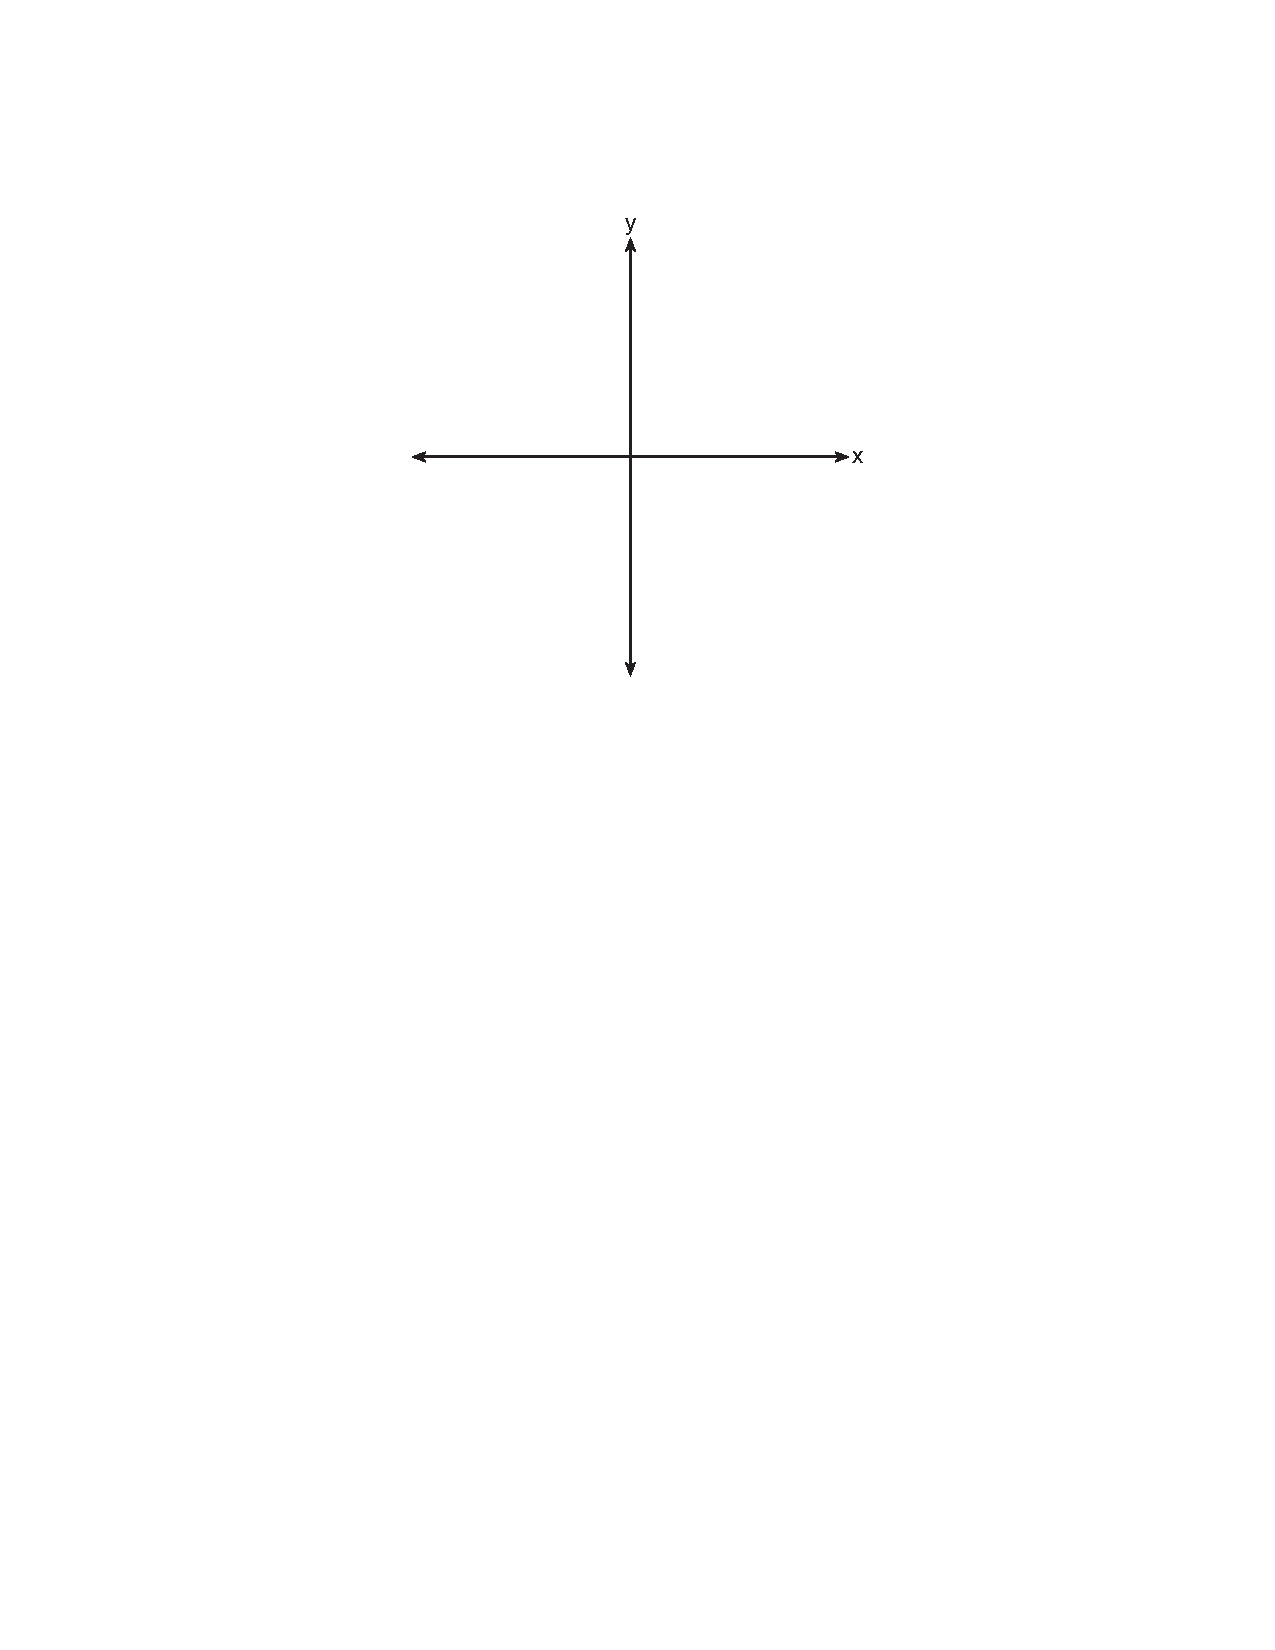
\includegraphics[width=0.5\textwidth]{simple-axes.pdf}
\end{figure}
\end{enumerate}}

\newpage
\subsection*{Do Now 1.6: Interpreting Graphical Features}
%End behavior
\begin{enumerate}
  \item
\end{enumerate}

\newpage
\subsection*{Homework 1.6: Cummulative Algebra Review}
\begin{enumerate}
  \item
\end{enumerate}


\newpage
\subsection*{Do Now 1.7: Simplifying Exponents}
\begin{enumerate}
  \item
  \item %2 points Aug 2017
  % Note that answer including text explanation is required
  Explain how $(-8)^\frac{4}{3}$ can be evaluated using properties of rational exponents to result in an integer answer.

  \item %2 points #31 June 2017
  Write $\sqrt[3]{x} \cdot \sqrt{x}$ as a single term with a rational exponent.

  \item %Multiple choice #23 Aug 2017
  What does $\displaystyle \left( \frac{-54x^9}{y^4}\right)^{\frac{2}{3}}$ equal?

  %\item %this is the multiple choice answer to the previous question
  %Simplify and express with rational exponents \[ \frac{9x^6 %\sqrt[3]{4}}{y^2 \sqrt[3]{y^2}}\]
\end{enumerate}


\newpage
\subsection*{Homework 1.7: Review}
\begin{enumerate}
  \item
  \emph{Spicy}
  \item %2 points #29 Aug 2017
  While experimenting with her calculator, Candy creates the sequence 4, 9, 19, 39, 79, $\ldots$.\\*[10 pt]
  Write a recursive formula for Candy's sequence.\\*[10 pt]
  Determine the eighth term in Candy's sequence.

  \item %4 points #34 Aug 2017
  Simon lost his library card and has an overdue library book. When the book was 5 days late, he owed \$2.25 to replace his library card and pay the fine for the overdue book. When the book was 21 days late, he owed \$6.25 to replace his library card and pay the fine for the overdue book.\\*[5 pt]
  Suppose the total amount Simon owes when the book is $n$ days late can be determined by an arithmetic sequence. Determine a formula for $a_n$, the $n$th term of this sequence.\\*[5 pt]
  Use the formula to determine the amount of money, in dollars, Simon needs to pay when the book is 60 days late.


\end{enumerate}


\newpage
\subsection*{Do Now 1.8: Graphing Exponential Functions}
%Classwork handout problems?
\begin{enumerate}

  \item %2 points #30 Aug 2017
  In New York State, the minimum wage has grown exponentially. In 1966, the minimum wage was \$1.25 an hour and in 2015, it was \$8.75. Algebraically determine the rate of growth to the \textit{nearest percent}.

  \item %4 points #30 June 2017
  Jim is looking to buy a vacation home for \$172,600 near his favorite southern beach. The formula to compute a mortgage payment, $M$, is $\displaystyle M=P \cdot \frac{r(1+r)^N}{(1+r)^N-1}$ where $P$ is the principal amount of the loan, $r$ is the monthly interest rate, and $N$ is the number of monthly payments. Jim's bank offers a monthly interest rate of 0.305\% for a 15-year mortgage.\\*[5pt]
  With no down payment, determine Jim's mortgage payment, rounded to the nearest dollar.\\*[5pt]
  Algebraically determine and state the down payment, rounded to the nearest dollar, that Jim needs to make in order for his mortgage payment to be \$1100.

  \item %6 points #37 June 2017
  A radioactive substance has a mass of 140 g at 3 p.m. and 100 g at 8 p.m. Write an equation in the form $\displaystyle A = A_0 \left( \frac{1}{2}\right) ^\frac{t}{h}$ that models this situation, where $h$ is the constant representing the number of hours in the half-life, $A_0$ is the initial mass, and $A$ is the mass $t$ hours after 3 p.m.\\*[10pt]
  Using this equation, solve for $h$, to the \textit{nearest ten thousandth}.\\*[10pt]
  Determine when the mass of the radioactive substance will be 40 g. Round your answer to the \textit{nearest tenth of an hour}.

  \newpage %necessary to keep grid with question
  \item %6 points #37 Aug 2017
  The value of a certain small passenger car based on its use in years is modeled by $V(t) =28482.698(0.684)^t$,
  where $V(t)$ is the value in dollars and $t$ is the time in years.
  Zach had to take out a loan to purchase the small passenger car. The function $Z(t) = 22151.327(0.778)^t$, where $Z(t)$ is measured in dollars,
  and $t$ is the time in years, models the unpaid amount of Zach's loan over time.\\*[10pt]
  Graph $V(t)$ and $Z(t)$ over the interval $0 \leq t \leq 5$, on the set of axes below.

  \begin{figure}[!ht]
      \centering
      
\includegraphics[width=0.6\textwidth]{1stQ-grid.pdf}
  \end{figure}

  State when $V(t) = Z(t)$, to the \textit{nearest hundredth}, and interpret its meaning in the context of the problem.\\*[10pt]
  Zach takes out an insurance policy that requires him to pay a \$3000 deductible in case of a collision. Zach will cancel the collision policy when the value of his car equals his deductible.
  To the nearest year, how long will it take Zach to cancel this policy? Justify your answer.
\end{enumerate}


\newpage
\subsection*{Homework 1.8: Pretest Study Questions}
\begin{enumerate}
  \item
  \newpage %necessary to place the grid following the text
  \item  %2 points #29 June 2017
  Graph $y =400(.85)^{2x} -6$ on the set of axes below.

  \begin{figure}[!ht]
      \centering
      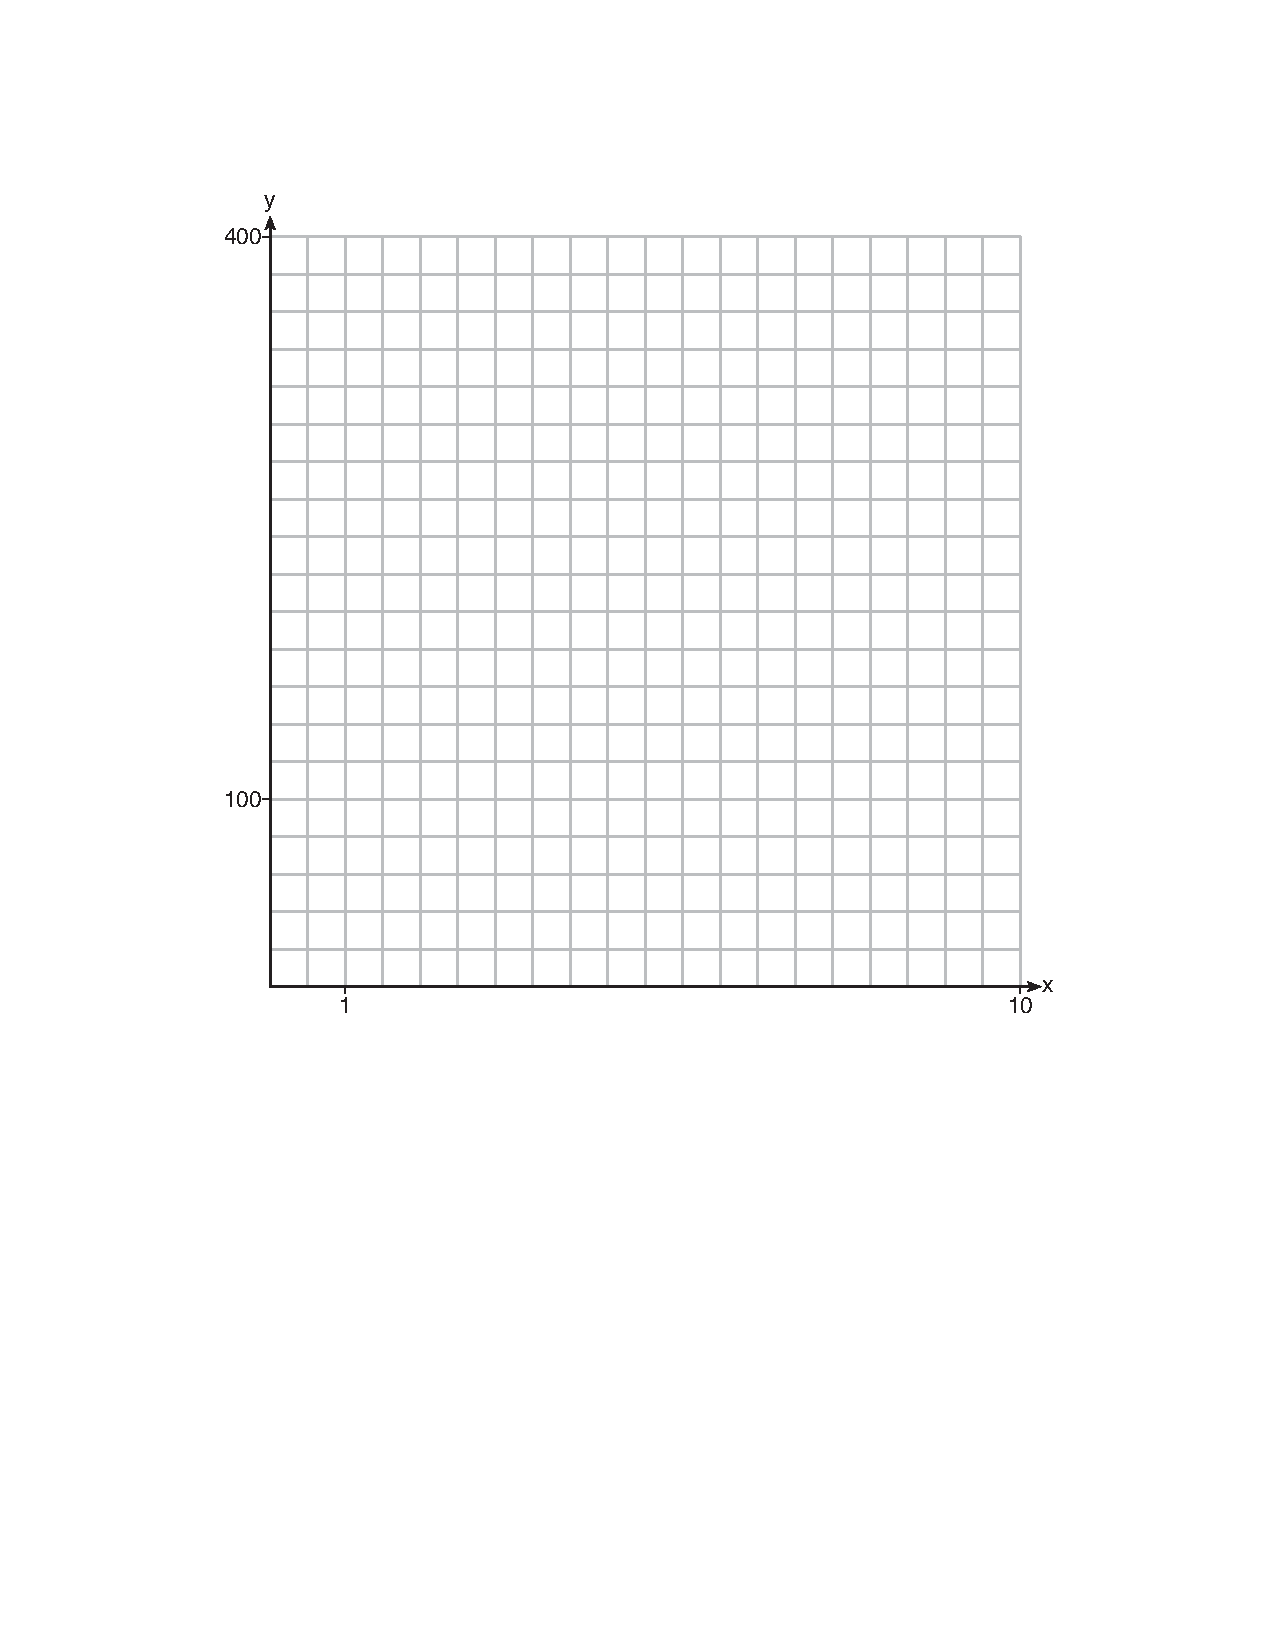
\includegraphics[width=0.85\textwidth]{1stQ-grid-special.pdf}
  \end{figure}

  \newpage %necessary to place the grid following the text
  \item  %4 points #35 June 2017
  Graph $y=log_2{(x +3)} - 5$ on the set of axes below. Use an appropriate scale to include \textit{both} intercepts.
  \vspace{0.5 in}
  \begin{figure}[!ht]
      \centering
      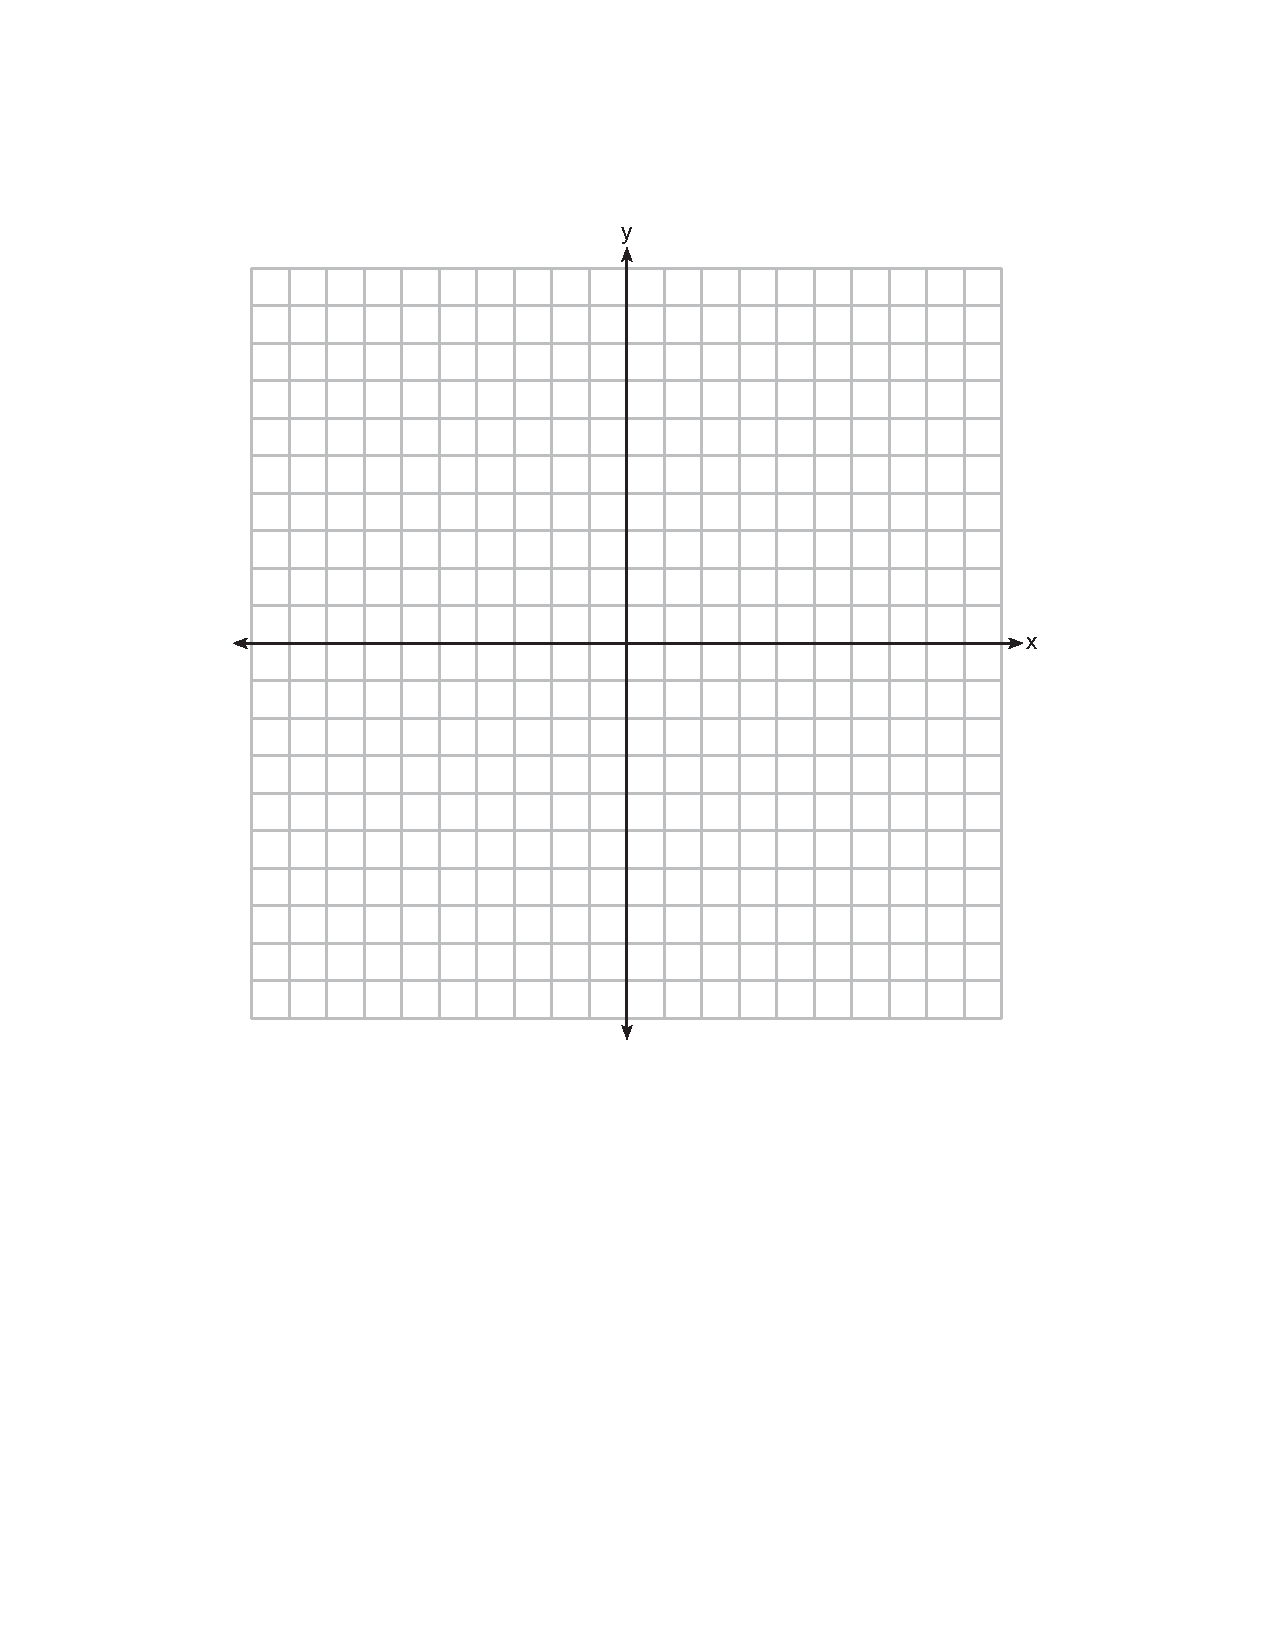
\includegraphics[width=0.75\textwidth]{regents-grid.pdf}
  \end{figure}

  Describe the behavior of the given function as $x$ approaches $-3$ and as $x$ approaches positive infinity.
\end{enumerate}


\newpage
\subsection*{Homework 1.10: Calculus Preparation}
\begin{enumerate}
  \item
\end{enumerate}

\end{document}
